\section{変更}
変更したら青文字.削除されたものは赤文字で表示される.

\section{algorithm}
\begin{algorithmic}
    \Function{hello world}{} 
    \State $str \gets "hello world"$
    \For{$s$ in $str$}
        \State{print($s$)}
    \EndFor
    \EndFunction
\end{algorithmic}

\section{画像}

\begin{figure}[t]
    \centering
    \includegraphics[width=\linewidth]{images/gnuplot_func.eps}
    \caption{gnuplot関数テスト}
    \label{fig:func}
\end{figure}

\begin{figure}[t]
    \centering
    \includegraphics[width=8cm]{images/replot.pdf}
    \caption{fragmasterテスト}
    \label{fig:fragmaster}
\end{figure}

\begin{figure}[t]
    \centering
    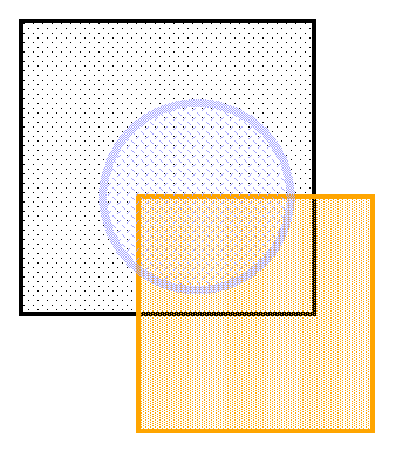
\includegraphics[width=10cm]{images/sample.eps}
    \caption{tgifテスト}
    \label{fig:tgif}
\end{figure}

\section{BibTex}
URL\cite{sagaweb}を参照